\chapter{Methods}
\label{ch:methods}

\section{Graph Representation}
\label{sec:graph-representation}

The current implementation represents a Grid2Op observation as a homogeneous,
directed graph whose nodes correspond to busbars and whose edges describe
possible transmission-line connections. Grid2Op exposes the instantaneous
electrical state and topology through a structured observation
\cite{donnot2020grid2op}. The graph construction maps this observation to
fixed-size tensors suitable for batched graph neural network training. Its main
design choice is to keep the set of candidate nodes and edges fixed throughout
an episode while using a dynamic edge mask to express the topology that is
electrically active at time step~$t$.

For agent~$a$, the graph observation can be written as
\begin{equation}
  \mathcal{G}^{(a)}_t =
  \left(\mathcal{V}^{(a)},\mathcal{E}^{(a)}_{\mathrm{cand}},
  \mathbf{X}^{(a)}_t,\mathbf{Z}^{(a)}_t,\mathbf{m}^{(a)}_t\right),
  \label{eq:agent-graph-observation}
\end{equation}
where $\mathcal{V}^{(a)}$ and
$\mathcal{E}^{(a)}_{\mathrm{cand}}$ are static, $\mathbf{X}^{(a)}_t$ contains
node features, $\mathbf{Z}^{(a)}_t$ contains edge features, and
$\mathbf{m}^{(a)}_t$ indicates which candidate edges are active. This separates
the physical equipment layout, which does not change during an episode, from
the busbar assignment and line status, which can change after every topology
action.

Figure~\ref{fig:busbar-graph-representation} illustrates this baseline schema:
busbars are the only nodes, while active transmission lines form the graph
backbone.

\begin{figure}[htbp]
  \centering
  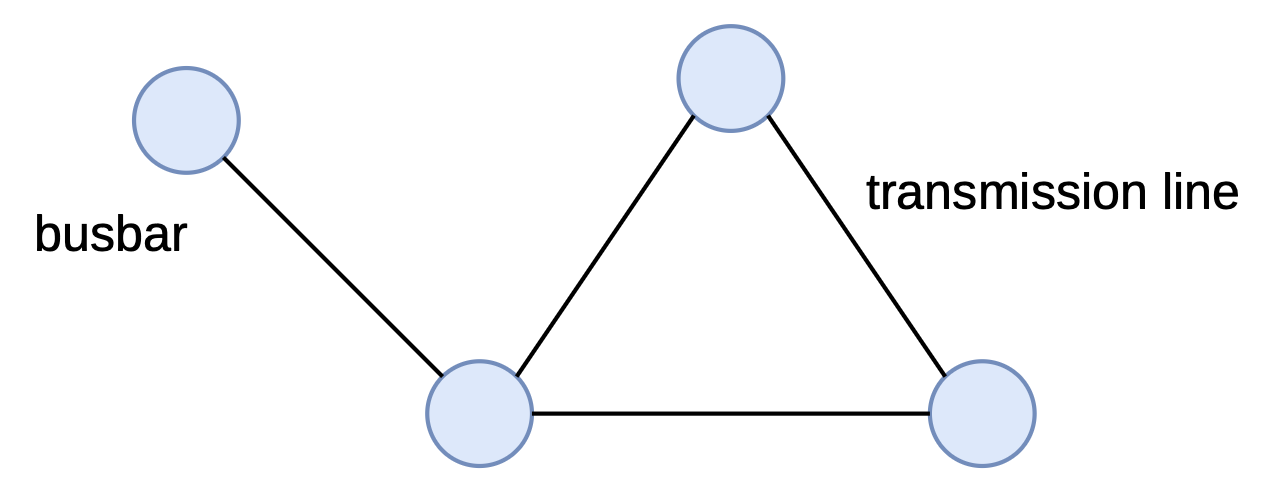
\includegraphics[width=0.94\linewidth]{figures/graph_busbar_baseline.png}
  \caption{Busbar graph representation. Blue nodes denote busbars and black
  connections denote active transmission-line relations. Generator and load
  quantities are aggregated into the features of their associated busbars.}
  \label{fig:busbar-graph-representation}
\end{figure}

\subsection{Busbar nodes}
\label{subsec:graph-busbar-nodes}

Let $S$ denote the number of substations and let $B$ denote the maximum number
of busbars per substation. A node is created for every substation--busbar pair,
including busbars to which no asset is connected at the current time. A global
node identifier is assigned as
\begin{equation}
  i(s,b)=sB+b,
  \qquad s\in\{0,\ldots,S-1\},\quad
  b\in\{0,\ldots,B-1\}.
  \label{eq:busbar-node-id}
\end{equation}
The complete graph therefore contains $SB$ nodes. Grid2Op uses one-based
busbar identifiers in its topology vector; these identifiers are converted to
the zero-based index $b$ in Equation~\ref{eq:busbar-node-id}.

Table~\ref{tab:graph-node-features} lists the six node features used in the
current representation. Generator and load quantities are assigned to the
busbar specified by the current topology vector. Active powers are summed when
several assets occupy the same busbar, whereas the corresponding angles are
averaged. Disconnected assets do not contribute to any node. The substation
cooldown is repeated on every busbar node of that substation.

\begin{table}[H]
  \centering
  \small
  \caption{Features attached to each busbar node.}
  \label{tab:graph-node-features}
  \setlength{\tabcolsep}{5pt}
  \begin{tabular}{L{0.28\textwidth}L{0.62\textwidth}}
    \toprule
    Feature & Definition \\
    \midrule
    \texttt{gen\_p} & Sum of active generator power connected to the busbar. \\
    \texttt{gen\_theta} & Mean voltage angle of generators connected to the busbar. \\
    \texttt{load\_p} & Sum of active load power connected to the busbar. \\
    \texttt{load\_theta} & Mean voltage angle of loads connected to the busbar. \\
    \texttt{time\_before\_cooldown\_sub} & Remaining substation cooldown. \\
    \texttt{domain\_mask} & One for a substation controlled by the agent and zero for a contextual neighbor. \\
    \bottomrule
  \end{tabular}
\end{table}

This aggregation produces a compact representation but deliberately removes
the identities and counts of individual generators and loads. Consequently,
two collections of assets with identical aggregated values have the same node
representation.

\subsection{Candidate line edges and dynamic topology}
\label{subsec:graph-candidate-edges}

Consider a physical line~$\ell$ whose origin and extremity belong to
substations $o(\ell)$ and $e(\ell)$. For every pair of possible endpoint
busbars $(b_o,b_e)$, the graph reserves the two directed candidate edges
\begin{equation}
  i(o(\ell),b_o)\rightarrow i(e(\ell),b_e)
  \quad\text{and}\quad
  i(e(\ell),b_e)\rightarrow i(o(\ell),b_o).
  \label{eq:candidate-line-edges}
\end{equation}
Thus, each physical line contributes $2B^2$ candidate directed edges. The two
directions share the same line attributes. For the usual case $B=2$, one line
produces eight candidate edges even though at most two---one per direction---are
electrically active at a given time.

The mask for a candidate endpoint assignment is
\begin{equation}
  m_{\ell,b_o,b_e,t}=
  \mathbf{1}\!\left[\text{line }\ell\text{ is connected at }t\right]
  \mathbf{1}\!\left[b^{\mathrm{or}}_{\ell,t}=b_o\right]
  \mathbf{1}\!\left[b^{\mathrm{ex}}_{\ell,t}=b_e\right].
  \label{eq:physical-edge-mask}
\end{equation}
If a line is disconnected, all of its candidate edges are masked. Otherwise,
only the pair corresponding to its current origin and extremity busbars remains
active. Inactive edge features are set to zero, and inactive edges are removed
before message passing. Topology changes can therefore modify graph connectivity
without changing tensor shapes or rebuilding the static graph specification.

The dynamic attributes copied onto active physical-line edges are given in
Table~\ref{tab:graph-edge-features}. The two maintenance features are present
only for environments with scheduled maintenance.

\begin{table}[H]
  \centering
  \small
  \caption{Features attached to physical-line edges.}
  \label{tab:graph-edge-features}
  \setlength{\tabcolsep}{5pt}
  \begin{tabular}{L{0.32\textwidth}L{0.58\textwidth}}
    \toprule
    Feature & Definition \\
    \midrule
    \texttt{line\_status} & Binary connection status of the physical line. \\
    \texttt{rho} & Line loading relative to its thermal limit. \\
    \texttt{timestep\_overflow} & Number of consecutive time steps in overload. \\
    \texttt{time\_before\_cooldown\_line} & Remaining cooldown before another line action is legal. \\
    \texttt{time\_next\_maintenance} & Time until scheduled maintenance, when available. \\
    \texttt{duration\_next\_maintenance} & Duration of scheduled maintenance, when available. \\
    \bottomrule
  \end{tabular}
\end{table}

\subsection{Physical scaling and running normalization}
\label{subsec:graph-feature-normalization}

Two optional preprocessing stages are implemented for every graph schema. They
are controlled independently with
\begin{center}
  \texttt{gnn\_physical\_scaling = true},
  \qquad
  \texttt{gnn\_running\_norm = true}.
\end{center}
Both options default to false so that historical experiments and checkpoints
retain their original inputs. When enabled together, deterministic physical
scaling is applied first and running standardization is applied second. The GNN
input is therefore
\begin{equation}
  \widehat{x}_{i,f,t}
  =
  \operatorname{clip}
  \left(
    \frac{x_{i,f,t}/s_f-\mu_{f,t}}
         {\sqrt{\sigma_{f,t}^{2}+\epsilon}},
    -c,c
  \right),
  \label{eq:graph-feature-normalization}
\end{equation}
for a continuous feature $f$ with physical scale $s_f$, running mean
$\mu_{f,t}$, running variance $\sigma_{f,t}^{2}$, and clipping threshold $c$.
The default is $c=10$, configurable through \texttt{gnn\_norm\_clip}. A
non-positive value disables clipping.

The first stage converts physical quantities to dimensionless ranges while
preserving a physical zero as zero. Table~\ref{tab:graph-physical-scales}
summarizes the implemented factors. The power base can be specified explicitly
with \texttt{gnn\_power\_scale\_mw}. When its value is non-positive, the
largest installed generator rating is used, with a 100~MW fallback when the
environment does not expose generator ratings.

\begin{table}[H]
  \centering
  \small
  \caption{Deterministic physical scales used for continuous graph features.}
  \label{tab:graph-physical-scales}
  \setlength{\tabcolsep}{5pt}
  \begin{tabular}{L{0.34\textwidth}L{0.25\textwidth}L{0.31\textwidth}}
    \toprule
    Features & Scale $s_f$ & Source \\
    \midrule
    \texttt{gen\_p}, \texttt{load\_p}, \texttt{p}
      & Power base in MW & Configured value or maximum generator rating. \\
    \texttt{gen\_theta}, \texttt{load\_theta}, \texttt{theta}
      & $180$ degrees & Fixed angular scale. \\
    \texttt{time\_before\_cooldown\_sub}
      & Maximum substation cooldown & Grid2Op environment parameter. \\
    \texttt{time\_before\_cooldown\_line}
      & Maximum line cooldown & Grid2Op environment parameter. \\
    \texttt{timestep\_overflow}
      & Allowed overflow duration & Grid2Op environment parameter. \\
    Maintenance time and duration
      & Episode horizon & Grid2Op chronic horizon. \\
    \bottomrule
  \end{tabular}
\end{table}

The loading ratio \texttt{rho} is already dimensionless and is not rescaled or
standardized. Preserving it is also necessary when GCN uses \texttt{rho}
directly as a non-negative message weight. Binary connection states, node and
edge masks, domain masks, type indicators, and relation one-hot attributes are
also left unchanged.

The second stage maintains Welford running statistics over the physically
scaled values. One shared normalizer serves every agent. At each environment
step, its statistics are updated once from the full state graph rather than
from every local graph; duplicated regional observations therefore do not
receive extra weight. Heterogeneous graphs maintain a separate node statistic
for each node type, preventing the structurally zero entries of busbars,
generators, loads, and transmission-line nodes from contaminating one another.
Edge statistics include only active physical-line relations. Inactive candidate
edges and self, asset-attachment, same-substation, and virtual relations do not
contribute.

Each parallel environment worker maintains local online statistics. Before
evaluation and checkpointing, the workers are merged using the parallel
Welford equations. The merged state is broadcast to evaluation environments,
saved in the checkpoint, restored when training resumes, and frozen during
evaluation. If running normalization is requested for standalone evaluation
but the checkpoint does not contain statistics, the existing normalization
policy either raises an error or disables the running stage according to the
selected evaluation mode.

This input normalization is distinct from the LayerNorm operations inside the
encoder. Equation~\ref{eq:graph-feature-normalization} gives a stable meaning
to each physical input channel, whereas LayerNorm acts on the learned hidden
channels of each individual node or edge after projection. Both stages can
therefore remain enabled simultaneously.

\subsection{Additional relation edges}
\label{subsec:graph-relation-edges}

The graph schema distinguishes three directed edge relations:
\emph{self}, \emph{physical line}, and \emph{same-substation busbar}. The
same-substation relation can be enabled for every encoder and graph
representation with
\begin{center}
  \texttt{gnn\_add\_substation\_edges = true}.
\end{center}
For each substation it adds a directed edge for every ordered pair of distinct
busbars. These edges remain active throughout the episode, carry zero-valued
physical-line features except for the neutral \texttt{rho} message weight, and
are distinguished by a categorical edge type. When the general option is left
unset, the existing behavior is preserved: same-substation and self relations
are enabled by default for the sparse graph transformer and disabled by default
for the other encoders.

Same-substation edges are computational attention relations; they do not imply
that the two busbars are electrically connected. They allow information to pass
between alternative busbar states within a substation, while edge-type
embeddings and relation-specific attention biases allow the encoder to treat
them differently from transmission lines. In the heterogeneous schemas, GAT
and GINE also receive the relation one-hot attribute. GCN and GraphSAGE use the
additional connectivity and identify the endpoints through their node
features.

\begin{figure}[htbp]
  \centering
  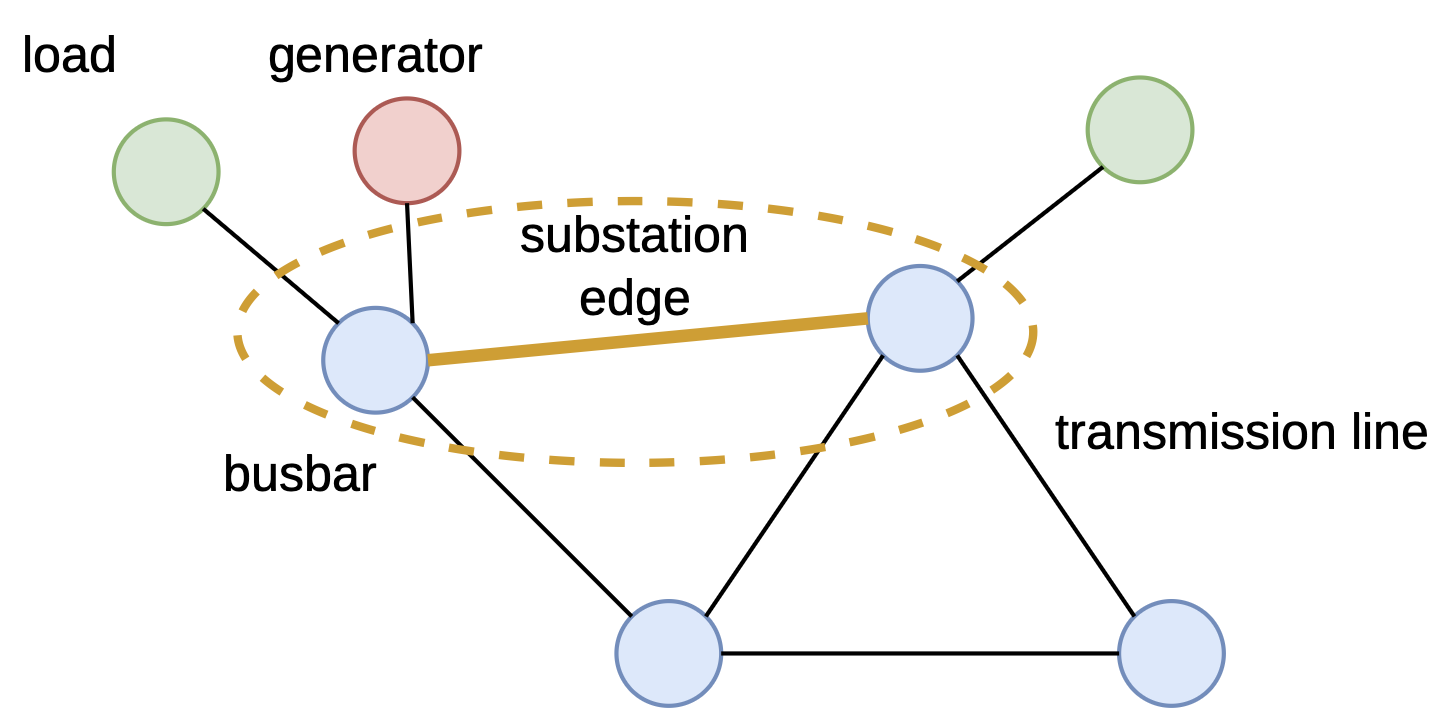
\includegraphics[width=0.94\linewidth]{figures/graph_same_substation_edge.png}
  \caption{Direct same-substation busbar relation. The highlighted orange edge
  allows two busbars belonging to the same substation to exchange messages; it
  is a computational relation and not a physical transmission line.}
  \label{fig:same-substation-busbar-edge}
\end{figure}

For a full graph containing $S$ substations and $L$ physical lines, the number
of candidate directed edges is
\begin{equation}
  |\mathcal{E}_{\mathrm{cand}}| = 2B^2L
  \label{eq:standard-graph-size}
\end{equation}
for the standard representation, and
\begin{equation}
  |\mathcal{E}_{\mathrm{cand}}| =
  2B^2L + SB + SB(B-1)
  \label{eq:sparse-transformer-graph-size}
\end{equation}
when self and same-substation relations are both enabled. As an illustration,
a 14-substation, 20-line system with two busbars has 28 nodes and 160 physical
candidate edges. Adding both relation types gives 216 candidate edges in total.

\subsection{Local actor graphs and the global state graph}
\label{subsec:graph-local-global}

Each agent controls a set of substations $\mathcal{C}_a$. Under decentralized
observability, its local graph can be constructed in two ways. Without neighbor
context, the node set contains only substations in $\mathcal{C}_a$, and the line
set contains only lines whose two endpoints lie inside this region. With
one-hop context enabled, the graph additionally contains every line touching
$\mathcal{C}_a$ and the substations at the opposite endpoints of those lines.
The \texttt{domain\_mask} node feature and a separate controlled-node mask
distinguish the controlled region from contextual neighbors. This second mask
also permits graph readout to pool only the nodes on which the agent can act.

Alongside every local graph, the environment constructs a full-grid
\emph{state graph}. A graph-based actor consumes its agent-specific local graph,
whereas a graph-based centralized critic consumes the state graph. This follows
the centralized-training, decentralized-execution structure of MAPPO
\cite{yu2022mappo}: actors can be restricted to regional information while the
critic uses a global representation during training.

The observation delivered to each agent has the conceptual structure
\begin{equation}
  \left\{
  \texttt{flat},\ \texttt{graph},\ \texttt{state\_graph}
  \right\}.
  \label{eq:structured-agent-observation}
\end{equation}
The local and state graphs each contain node features, edge features, node and
edge masks, edge types, and a controlled-node mask. Their static specifications,
including node identifiers and candidate edge indices, are built once when the
environment is initialized.

\subsection{Boundary between representation and encoder}
\label{subsec:graph-representation-encoder-boundary}

The busbar graph is shared by several encoder architectures. GAT and GINE use
the edge attributes directly; GCN can optionally use \texttt{rho} as an edge
weight; GraphSAGE uses the active connectivity without edge attributes; and the
sparse graph transformer can use both continuous edge attributes and categorical
edge relations. Optional learned substation and busbar embeddings may be
concatenated to the node features. After message passing, the node embeddings
are pooled into one fixed-dimensional graph embedding. This embedding can be
used alone or concatenated with the original flat observation before it enters
the actor or critic head.

These choices change how the graph is encoded, but not which physical entities
the graph represents. The busbar schema does not create separate generator,
load, line, or substation nodes, and it does not encode reactive power, voltage
magnitudes, or directional endpoint flows. Empty busbars remain in the node
set, and the node mask is currently one for every allocated node. Moreover,
graph features are taken from the raw Grid2Op observation by default. The
optional physical scaling and shared running normalization from
Section~\ref{subsec:graph-feature-normalization} can be enabled without changing
the graph schema. These properties define the busbar baseline against which the
heterogeneous representation introduced next can be compared.

\section{Heterogeneous Graph Representation}
\label{sec:heterogeneous-graph-representation}

The second representation makes the equipment categories explicit instead of
aggregating generators and loads into busbar features. It follows the structure
illustrated conceptually by a network in which busbars form the blue backbone,
generators are red terminal nodes, and loads are green terminal nodes. The graph
contains three node types,
\begin{equation}
  \mathcal{V} =
  \mathcal{V}_{\mathrm{bus}}
  \cup \mathcal{V}_{\mathrm{gen}}
  \cup \mathcal{V}_{\mathrm{load}},
  \label{eq:heterogeneous-node-set}
\end{equation}
and typed directed relations between them. This preserves the identity and
state of every generator and load while retaining the busbar-level description
of the controllable topology.

\begin{figure}[htbp]
  \centering
  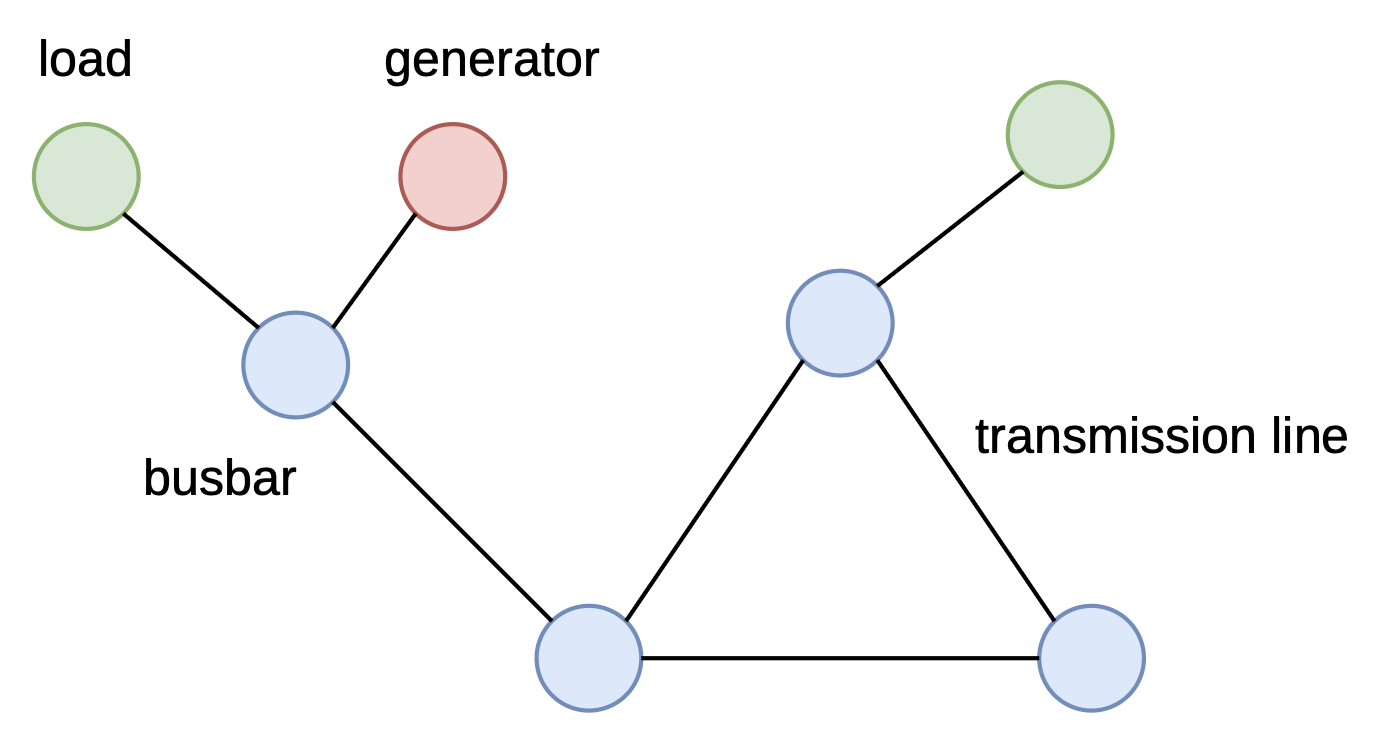
\includegraphics[width=0.92\linewidth]{figures/graph_heterogeneous_equipment.png}
  \caption{Heterogeneous equipment representation. Busbars are blue, generators
  are red, and loads are green. Physical transmission lines remain direct
  relations between busbar nodes.}
  \label{fig:heterogeneous-equipment-graph}
\end{figure}

The implementation is selected with
\texttt{gnn\_graph\_type = heterogeneous}. It uses the same local actor and
global state-graph interface as the busbar representation, so the graph schema
can be changed without modifying MAPPO rollout collection or the actor and
critic APIs.

\subsection{Typed nodes and features}
\label{subsec:heterogeneous-nodes}

For a graph with $S$ included substations, $B$ busbars per substation, $N_g$
included generators, and $N_d$ included loads, the number of nodes is
\begin{equation}
  |\mathcal{V}| = SB + N_g + N_d.
  \label{eq:heterogeneous-node-count}
\end{equation}
Busbar nodes are created exactly as in
Section~\ref{subsec:graph-busbar-nodes}. In addition, each generator and load
whose substation is present in the graph receives its own node. Asset nodes
remain allocated when an asset is disconnected, thereby preserving fixed tensor
shapes throughout an episode.

All node types are stored in one feature matrix. Type-specific values occupy a
shared feature schema, with unused entries set to zero. Table~\ref{tab:heterogeneous-node-features}
lists this schema.

\begin{table}[H]
  \centering
  \small
  \caption{Unified node features in the heterogeneous representation.}
  \label{tab:heterogeneous-node-features}
  \setlength{\tabcolsep}{5pt}
  \begin{tabular}{L{0.30\textwidth}L{0.60\textwidth}}
    \toprule
    Feature & Definition \\
    \midrule
    \texttt{is\_busbar} & One for busbar nodes and zero otherwise. \\
    \texttt{is\_generator} & One for generator nodes and zero otherwise. \\
    \texttt{is\_load} & One for load nodes and zero otherwise. \\
    \texttt{p} & Generator active production or load active consumption. \\
    \texttt{theta} & Generator or load voltage angle. \\
    \texttt{time\_before\_cooldown\_sub} & Substation cooldown on busbar nodes. \\
    \texttt{connected} & One for busbars and for currently connected assets; zero for a disconnected asset. \\
    \texttt{domain\_mask} & One when the node belongs to a substation controlled by the agent. \\
    \bottomrule
  \end{tabular}
\end{table}

When an asset is disconnected, its \texttt{connected} feature becomes zero and
its dynamic \texttt{p} and \texttt{theta} entries are zeroed. Its type and
substation identity remain available. Unlike the busbar representation,
generator and load values are not summed or averaged, so two assets connected
to the same busbar can retain different states.

\subsection{Typed relations}
\label{subsec:heterogeneous-relations}

The heterogeneous graph uses seven possible directed edge relations:
\begin{enumerate}
  \item \emph{self};
  \item \emph{physical line}, between two busbars;
  \item \emph{same-substation busbar};
  \item \emph{generator-to-busbar};
  \item \emph{busbar-to-generator};
  \item \emph{load-to-busbar};
  \item \emph{busbar-to-load}.
\end{enumerate}
Direction-specific asset relations allow an encoder to learn different
transformations for information entering and leaving a generator or load. Self
and same-substation relations remain optional and are enabled by default for the
sparse graph transformer, as in the busbar representation.

Physical transmission lines use the candidate endpoint construction from
Equation~\ref{eq:candidate-line-edges}. Asset attachments follow the same
fixed-shape principle. For generator $g$ located at substation $s(g)$, the
candidate set contains
\begin{equation}
  g \rightarrow i(s(g),b)
  \quad\text{and}\quad
  i(s(g),b) \rightarrow g,
  \qquad b\in\{0,\ldots,B-1\}.
  \label{eq:generator-busbar-candidates}
\end{equation}
Only the two directed edges associated with the generator's current busbar are
active. Loads are handled identically. If an asset is disconnected in the
topology vector, all of its attachment edges are masked. A topology action can
therefore move an asset from one busbar to another by changing masks, while the
candidate edge index remains static.

Without optional self and same-substation relations, the candidate edge count
is
\begin{equation}
  |\mathcal{E}_{\mathrm{cand}}| =
  2B^2L + 2B(N_g+N_d),
  \label{eq:heterogeneous-edge-count}
\end{equation}
where $L$ is the number of included physical lines. Enabling both optional
relations adds $|\mathcal{V}|$ self-edges and $SB(B-1)$ directed
same-substation busbar edges.

\subsection{Tensor representation and encoder compatibility}
\label{subsec:heterogeneous-tensors}

Semantically, the graph is heterogeneous because its nodes and relations have
different physical meanings. Operationally, it is represented using unified
tensors rather than separate PyTorch Geometric node stores. The observation adds
a categorical \texttt{node\_type} tensor and retains the categorical
\texttt{edge\_type} tensor. The three node-type indicators are also included in
the node feature matrix. Similarly, a one-hot relation block is appended to the
continuous edge attributes. This dual representation makes the schema usable by
the existing encoders:
\begin{itemize}
  \item GAT and GINE receive the relation one-hot values as edge attributes;
  \item the sparse graph transformer receives the integer relation identifiers
  through its relation embeddings and attention biases;
  \item GCN and GraphSAGE infer equipment roles from the node-type features,
  even though their standard layers do not directly consume edge types.
\end{itemize}

The physical-line part of the edge feature vector retains the attributes from
Table~\ref{tab:graph-edge-features}. Structural relations use a neutral unit
value in the \texttt{rho} position so they remain effective when GCN is
configured to use \texttt{rho} as a message weight; this value is a computational
weight rather than a physical loading ratio. Inactive candidate relations are
removed before message passing, exactly as for physical lines.

\subsection{Local heterogeneous graphs}
\label{subsec:local-heterogeneous-graphs}

The decentralized domain rules remain unchanged. A local graph first selects
its controlled substations and, optionally, their one-hop neighboring
substations. It then includes the busbars, generators, and loads belonging to
those substations, together with the selected physical lines. Consequently,
neighbor assets are available as context when one-hop expansion is enabled, but
the controlled-node mask still distinguishes them from equipment inside the
agent's action domain. The centralized state graph contains all busbars,
generators, loads, physical lines, and active attachment relations in the grid.

The principal trade-off is therefore explicitness against size. The busbar
representation is smaller but aggregates equipment values. The heterogeneous
representation introduces $N_g+N_d$ nodes and $2B(N_g+N_d)$ candidate
attachment edges, but preserves individual asset states and gives the encoder
typed paths that mirror the intended physical structure.

\section{Heterogeneous Graph with Transmission-Line Nodes}
\label{sec:heterogeneous-line-graph}

The third representation extends Section~\ref{sec:heterogeneous-graph-representation}
by representing every transmission line as a node rather than as a direct edge
between two busbars. In the conceptual diagram, busbars are blue, generators
are red, loads are green, and transmission lines are yellow. The line nodes
form the intermediate elements through which information passes between the
busbars at the two ends of each physical line. The resulting node set is
\begin{equation}
  \mathcal{V} =
  \mathcal{V}_{\mathrm{bus}}
  \cup \mathcal{V}_{\mathrm{gen}}
  \cup \mathcal{V}_{\mathrm{load}}
  \cup \mathcal{V}_{\mathrm{line}}.
  \label{eq:heterogeneous-line-node-set}
\end{equation}

\begin{figure}[htbp]
  \centering
  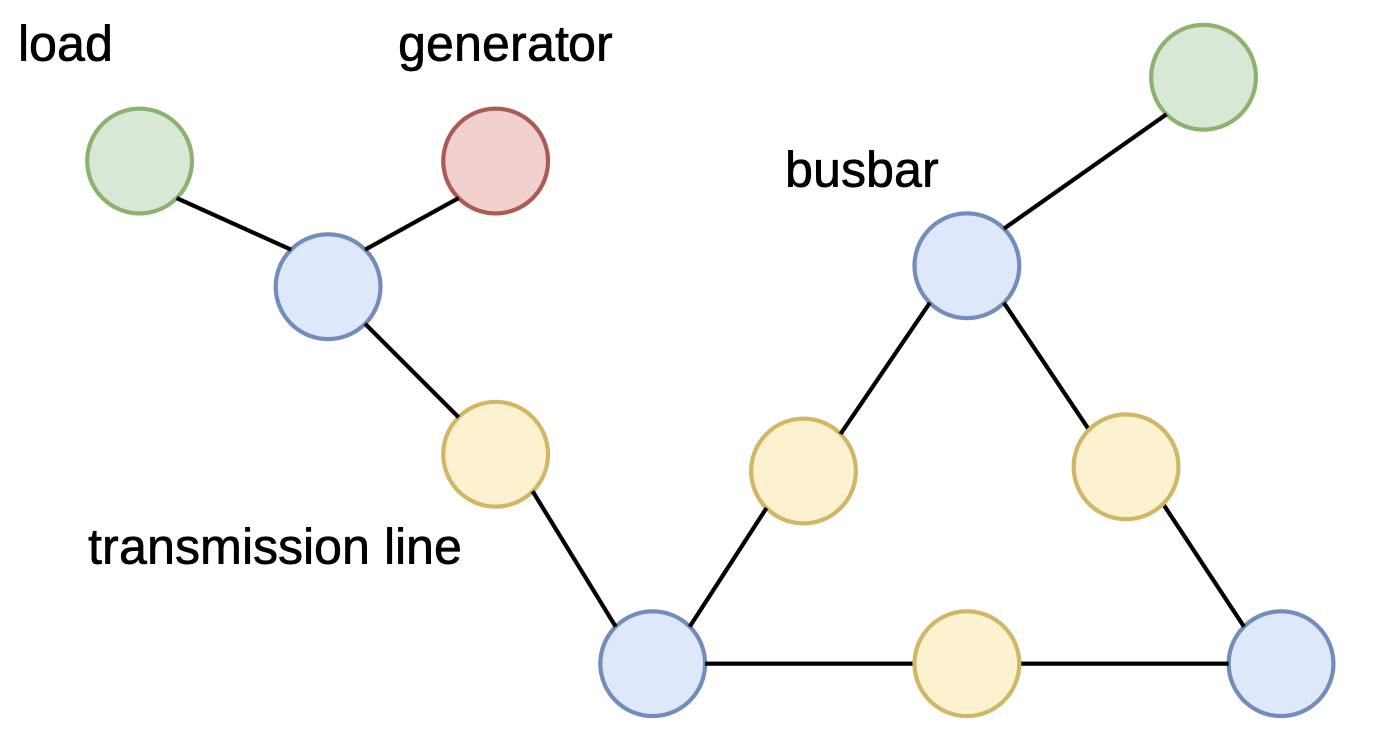
\includegraphics[width=0.92\linewidth]{figures/graph_heterogeneous_line_nodes.png}
  \caption{Heterogeneous representation with explicit transmission-line nodes.
  Yellow nodes represent physical lines and connect the blue busbars at their
  endpoints; generators and loads remain explicit terminal nodes.}
  \label{fig:heterogeneous-line-node-graph}
\end{figure}

This schema is selected with
\texttt{gnn\_graph\_type = heterogeneous\_line}. It implements the same fixed
tensor interface used by the two preceding representations and can therefore
be used by the existing GNN actor and critic encoders without changing the
MAPPO training loop.

\subsection{Node allocation and features}
\label{subsec:heterogeneous-line-nodes}

For $S$ included substations, $B$ busbars per substation, $N_g$ generators,
$N_d$ loads, and $L$ included transmission lines, the graph contains
\begin{equation}
  |\mathcal{V}| = SB + N_g + N_d + L
  \label{eq:heterogeneous-line-node-count}
\end{equation}
nodes. Busbar, generator, and load nodes retain the features described in
Table~\ref{tab:heterogeneous-node-features}. A fourth type indicator,
\texttt{is\_transmission\_line}, identifies line nodes. The unified node-feature
matrix additionally provides the line-specific state shown in
Table~\ref{tab:heterogeneous-line-node-features}; entries that do not apply to a
given node type are set to zero.

\begin{table}[H]
  \centering
  \small
  \caption{Features carried by an explicit transmission-line node.}
  \label{tab:heterogeneous-line-node-features}
  \setlength{\tabcolsep}{5pt}
  \begin{tabular}{L{0.34\textwidth}L{0.56\textwidth}}
    \toprule
    Feature & Definition \\
    \midrule
    \texttt{line\_status} & One when the physical line is connected and zero otherwise. \\
    \texttt{rho} & Line loading ratio. \\
    \texttt{timestep\_overflow} & Number of consecutive overflow time steps. \\
    \texttt{time\_before\_cooldown\_line} & Remaining line-reconnection cooldown. \\
    \texttt{time\_next\_maintenance} & Time until planned maintenance, when maintenance features are enabled. \\
    \texttt{duration\_next\_maintenance} & Planned maintenance duration, when maintenance features are enabled. \\
    \texttt{connected} & One for an online line and zero for a disconnected line. \\
    \texttt{domain\_mask} & One when either endpoint belongs to a substation controlled by the agent. \\
    \bottomrule
  \end{tabular}
\end{table}

A disconnected line remains allocated in the graph, so neither the node count
nor the candidate edge index changes during an episode. Its
\texttt{line\_status} and \texttt{connected} entries become zero and all of its
busbar attachments are masked. Other state, such as its cooldown and
maintenance timing, remains visible to the encoder. This distinction lets the
policy reason about a temporarily unavailable physical element without
mistaking it for an element that does not exist.

\subsection{Endpoint-specific typed relations}
\label{subsec:heterogeneous-line-relations}

Let $o(\ell)$ and $e(\ell)$ denote the origin and extremity substations of line
$\ell$. For every busbar index $b$, the fixed candidate graph contains
\begin{equation}
  i(o(\ell),b) \leftrightarrow \ell
  \qquad\text{and}\qquad
  i(e(\ell),b) \leftrightarrow \ell,
  \quad b\in\{0,\ldots,B-1\}.
  \label{eq:heterogeneous-line-candidates}
\end{equation}
The bidirectional symbol denotes two directed relations. At a particular time,
the topology vector activates only the origin and extremity busbars to which the
line is currently attached. Thus, an online line has four active directed
attachment edges: busbar-to-line and line-to-busbar at each endpoint. A topology
action only changes the edge mask; it does not rebuild the candidate graph.

The representation distinguishes ten relation types:
\begin{enumerate}
  \item self;
  \item same-substation busbar;
  \item busbar-to-line at the origin;
  \item line-to-busbar at the origin;
  \item busbar-to-line at the extremity;
  \item line-to-busbar at the extremity;
  \item generator-to-busbar;
  \item busbar-to-generator;
  \item load-to-busbar;
  \item busbar-to-load.
\end{enumerate}
Separating direction and line endpoint allows a relation-aware encoder to learn
different transformations for the two terminals of a transmission line. The
generator and load attachment rules are unchanged from
Equation~\ref{eq:generator-busbar-candidates}. Self and same-substation busbar
relations remain optional.

Without the optional relations, the number of candidate directed edges is
\begin{equation}
  |\mathcal{E}_{\mathrm{cand}}| =
  4BL + 2B(N_g+N_d).
  \label{eq:heterogeneous-line-edge-count}
\end{equation}
For the common case $B=2$, the line-attachment term has the same size as the
$2B^2L$ direct busbar-to-busbar candidate set in
Equation~\ref{eq:heterogeneous-edge-count}. For $B>2$, explicit line nodes make
this term grow linearly rather than quadratically with the number of busbars.

\subsection{Tensor representation and local graphs}
\label{subsec:heterogeneous-line-tensors}

As in the preceding heterogeneous representation, all node types share one
node-feature tensor. The categorical \texttt{node\_type} tensor has four values,
and the type indicators are also present in the node features. The categorical
\texttt{edge\_type} tensor identifies the ten relations, while a corresponding
one-hot relation block is appended to the edge features for encoders such as
GAT and GINE. The line loading ratio is copied to active line-attachment edges
so it can also be used as a GCN message weight; non-line structural relations
receive a neutral unit weight. The complete physical line state remains
available principally on the line node.

Local actor graphs use the same domain and one-hop-neighbor selection as the
other schemas. An included line receives one line node and its candidate
attachments to the included busbars. A line node is marked as controlled when
at least one of its endpoints belongs to the agent's controlled domain. The
centralized state graph contains all busbar, generator, load, and transmission
line nodes. Compared with the direct-edge heterogeneous graph, this
representation adds $L$ nodes and an extra message-passing step between the two
endpoint busbars, but makes each transmission line an identifiable entity whose
state can be updated and embedded independently.

\section{Substation Summary Nodes}
\label{sec:substation-summary-nodes}

An optional hierarchical augmentation introduces one learned node for every
substation included in the graph. It is enabled with
\begin{center}
  \texttt{gnn\_add\_substation\_nodes = true}.
\end{center}
For substation $s$, let $u_s$ denote its summary node and let
$\mathcal{B}(s)$ be its included busbar nodes. The augmented graph contains the
bidirectional structural relations
\begin{equation}
  \mathcal{E}_{\mathrm{sub}} =
  \left\{
    (i,u_s),(u_s,i)
    \;\middle|\;
    i\in\mathcal{B}(s)
  \right\}.
  \label{eq:substation-node-edges}
\end{equation}
Each substation node therefore gathers information from every busbar belonging
to that substation and can redistribute its learned summary to those busbars in
later message-passing layers. It is not connected directly to generators,
loads, or transmission-line nodes; those elements influence it through their
busbar attachments.

\begin{figure}[htbp]
  \centering
  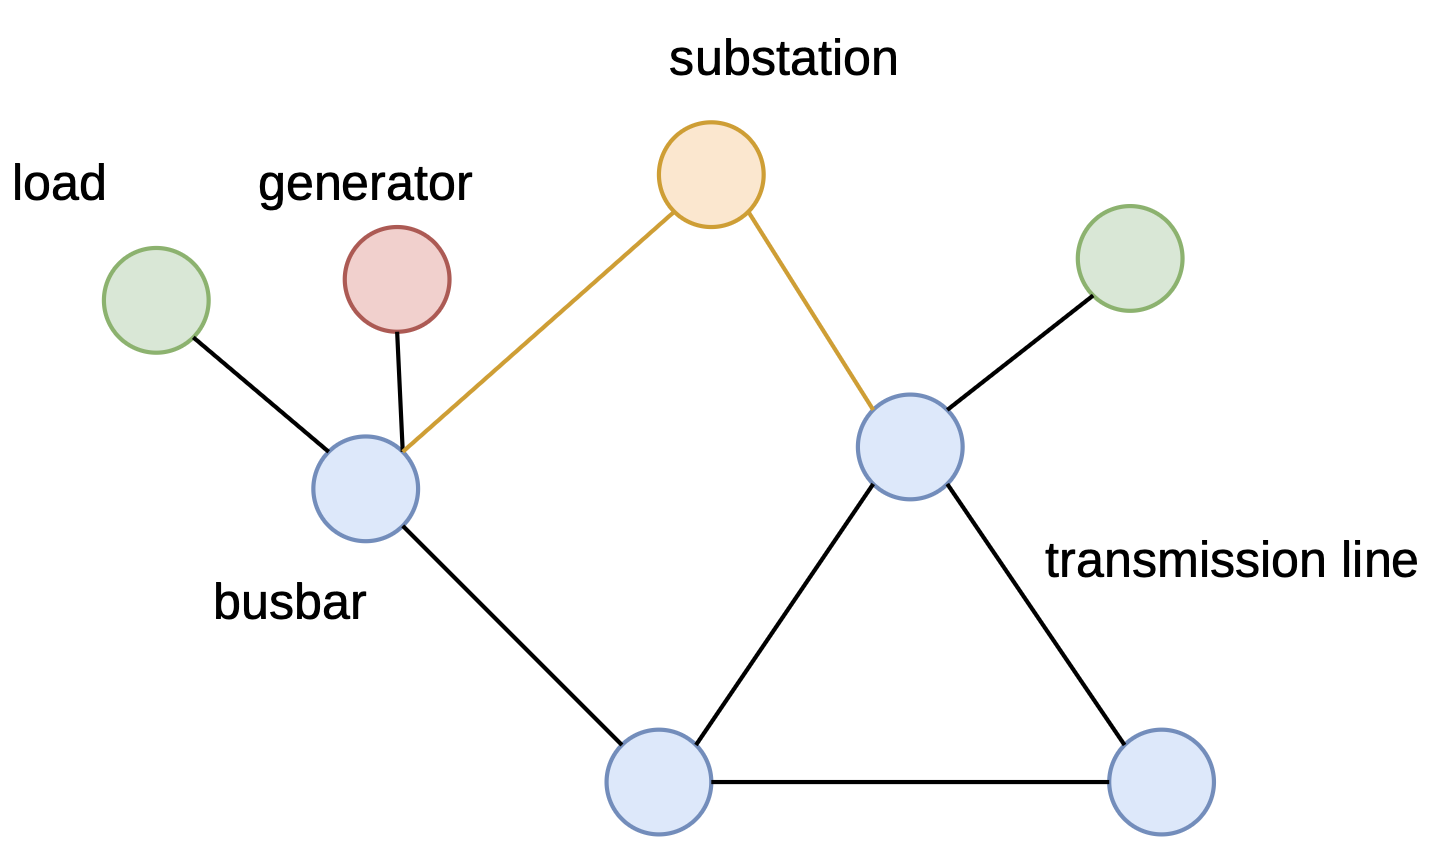
\includegraphics[width=0.88\linewidth]{figures/graph_substation_summary_node.png}
  \caption{Learned substation-summary augmentation. The orange substation node
  receives messages from each of its blue busbar nodes and can redistribute the
  resulting substation-level representation.}
  \label{fig:substation-summary-node}
\end{figure}

The initial substation-node states are learned embeddings indexed by the global
substation identifiers. For $S$ included substations and $B$ busbars per
substation, the augmentation adds $S$ nodes and $2SB$ directed edges. The nodes
are constructed inside the encoder, leaving the environment observation and
rollout-storage shapes unchanged. Standard mean, sum, maximum, or attention
readout includes the new summary nodes. Controlled readout marks a substation
node as controlled whenever at least one of its busbars is controlled. The
sparse graph transformer assigns the attachments a dedicated learned relation.

Substation nodes can also be combined with the virtual-node readout introduced
next. In that case, information follows a hierarchy from physical equipment to
busbars, from busbars to substation nodes, and from substation nodes to one
graph-level virtual node. The node augmentation is distinct from the direct
same-substation edges in Section~\ref{subsec:graph-relation-edges}: the former
introduces a learned hub $u_s$, whereas the latter directly connects pairs of
busbars. Either mechanism, or both, may be enabled.

\section{Virtual-Node Graph Readout}
\label{sec:virtual-node-readout}

The preceding graph representations normally produce a fixed-dimensional graph
embedding by applying mean, sum, maximum, or attention pooling after the final
message-passing layer. An alternative readout is implemented using one
\emph{virtual node}. This node acts as a learned summary of all substations in
the current graph and replaces the terminal pooling operation. The option is
selected with
\begin{center}
  \texttt{gnn\_readout\_aggr = virtual\_node}.
\end{center}
It is independent of the graph representation and can therefore be combined
with the busbar, heterogeneous, or heterogeneous-line schema.

\subsection{Augmented graph}
\label{subsec:virtual-node-augmented-graph}

Let $v_{\star}$ denote the virtual node. Define the summary set
$\mathcal{V}_{\mathrm{sum}}$ as the included substation nodes when the
augmentation from Section~\ref{sec:substation-summary-nodes} is enabled, and as
the included busbar nodes otherwise. At encoder runtime, the graph is augmented
as
\begin{align}
  \mathcal{V}^{+} &= \mathcal{V}\cup\{v_{\star}\}, \\
  \mathcal{E}^{+} &= \mathcal{E}\cup
  \left\{
    (i,v_{\star}),(v_{\star},i)
    \;\middle|\;
    i\in\mathcal{V}_{\mathrm{sum}}
  \right\}.
  \label{eq:virtual-node-augmentation}
\end{align}
Without substation summary nodes, the virtual node is connected bidirectionally
to every included busbar, as illustrated by the purple links in
Figure~\ref{fig:virtual-node-readout}. With the hierarchical augmentation
enabled, the virtual node instead
connects to every included substation node. It is never connected directly to
generator, load, or transmission-line nodes. Those entities nevertheless
influence it through their ordinary paths to the busbar backbone. Masked
busbar nodes do not receive hierarchy connections.

\begin{figure}[htbp]
  \centering
  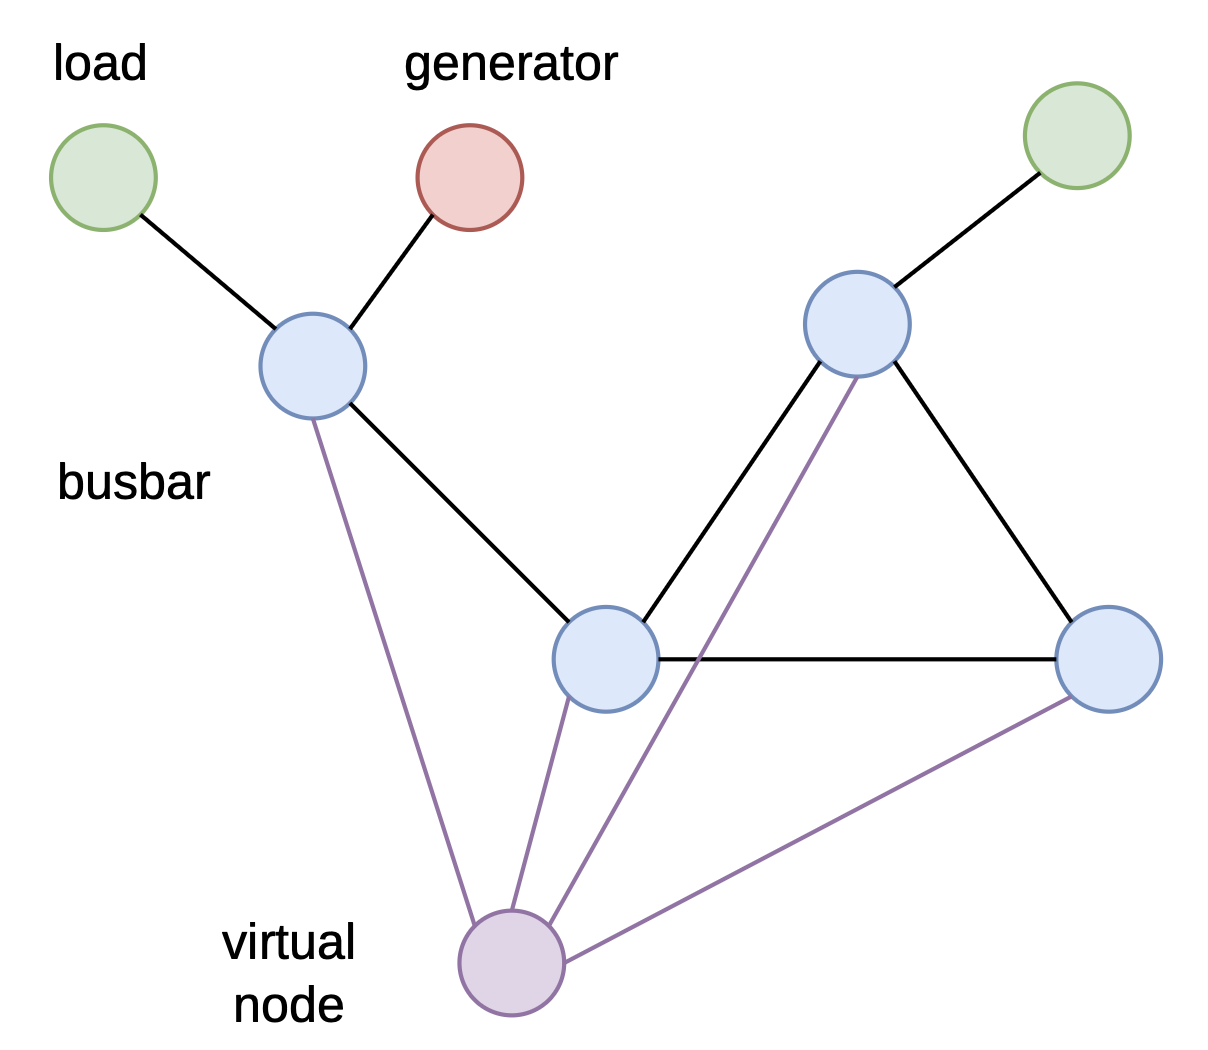
\includegraphics[width=0.68\linewidth]{figures/graph_virtual_node_readout.png}
  \caption{Virtual-node graph readout. The purple node exchanges messages with
  every included busbar and its final embedding replaces terminal node
  pooling. When substation-summary nodes are enabled, the virtual node connects
  to those summaries instead.}
  \label{fig:virtual-node-readout}
\end{figure}

The virtual node is appended inside the encoder rather than the environment.
Consequently, the Grid2Op observation tensors, static graph specifications, and
rollout storage retain their original dimensions. For a minibatch of $M$
graphs, the encoder creates $M$ independent copies of the virtual node and does
not introduce edges between different graphs.

\subsection{Learned summary instead of terminal pooling}
\label{subsec:virtual-node-summary}

The initial virtual representation $\mathbf{h}_{\star}^{(0)}$ is a learned
parameter shared across input graphs. Each graph receives a copy of this
parameter. Because the virtual edges are present during every layer, a generic
message-passing update jointly evolves the physical and virtual nodes:
\begin{equation}
  \left(
    \{\mathbf{h}_{i}^{(k+1)}\}_{i\in\mathcal{V}},
    \mathbf{h}_{\star}^{(k+1)}
  \right)
  =
  \operatorname{GNN}^{(k)}
  \left(
    \{\mathbf{h}_{i}^{(k)}\}_{i\in\mathcal{V}},
    \mathbf{h}_{\star}^{(k)},
    \mathcal{E}^{+}
  \right).
  \label{eq:virtual-node-update}
\end{equation}
Incoming busbar or substation messages let $v_{\star}$ accumulate a graph-level
summary, while the reverse edges let its current state influence the hierarchy
in subsequent layers. With $K$ layers, the graph embedding is obtained directly
from the final virtual state,
\begin{equation}
  \mathbf{z}_{G}
  = \operatorname{ReLU}
    \left(\mathbf{W}_{o}\mathbf{h}_{\star}^{(K)}+\mathbf{b}_{o}\right),
  \label{eq:virtual-node-readout}
\end{equation}
rather than from
$\operatorname{Pool}(\{\mathbf{h}_{i}^{(K)}\}_{i\in\mathcal{V}})$. The output
dimension and the actor--critic interface are therefore unchanged.

\subsection{Relation attributes and encoder compatibility}
\label{subsec:virtual-node-compatibility}

The readout is supported by GCN, GAT, GINE, GraphSAGE, and the sparse graph
transformer. Virtual connections are structural rather than physical: their
continuous edge attributes are zero, except for a neutral unit value in the
\texttt{rho} position when that feature exists. The unit value ensures that a
GCN configured to use \texttt{rho} as an edge weight does not suppress virtual
messages. The sparse graph transformer allocates dedicated learned relations
for substation attachments and virtual-node attachments, allowing its attention
layers to distinguish hierarchy links from all physical and equipment
relations.

Without substation nodes, a graph containing $N_{\mathrm{bus}}$ included
busbars receives one virtual node and $2N_{\mathrm{bus}}$ directed edges. With
the hierarchy enabled, the virtual-node stage instead adds $2S$ edges on top of
the substation augmentation. The method avoids a fixed, parameter-free
reduction such as mean or sum pooling, but its summary quality depends on
message-passing depth: after the first layer it has aggregated its immediate
busbar or substation neighbors, and later layers permit repeated interaction
between the summary and the physical graph. In a decentralized actor, the virtual node
summarizes the controlled domain together with any included one-hop context; in
the centralized critic, it summarizes the full state graph.

\section{Staged Graph-Architecture Screening Protocol}
\label{sec:graph-screening-protocol}

The representation, preprocessing, hierarchy, readout, and encoder choices
defined above form a large factorial design. Even when graph readout is limited
to mean pooling and the virtual node, a simultaneous sweep over three graph
schemas, four input-preprocessing modes, three binary structural factors, and
five encoders would require
\begin{equation}
  3 \times 4 \times 2^{3} \times 5 = 480
  \label{eq:full-graph-factorial}
\end{equation}
conditions before adding random seeds. The implemented screening therefore
uses sequential promotion: each stage varies one group of factors and inherits
the selected setting from the preceding stage. This reduces the initial screen
to 25 runs while retaining an explicit test of every proposed mechanism.

\subsection{Common screening controls}
\label{subsec:graph-screening-controls}

All screening runs first use the \texttt{bus14} environment, the same action
space, the same train--test chronic split, training seed zero, 72 parallel
environments, and rollouts of 576 steps. A run receives 8 million environment
steps, slightly more than half of the 15-million-step bus14 confirmation budget.
Evaluation is deterministic and uses the same held-out chronic set in every
condition. The smaller network makes the 25-run screen affordable before the
selected design is scaled to WCCI.

The actor uses a 128-dimensional, two-layer graph encoder followed by the same
action head in every condition. Two message-passing layers are necessary for a
fair evaluation of the explicit-line schema: information can travel from a
busbar to a line node and then to the opposite busbar. The critic is a fixed MLP,
so the screen measures changes to the actor graph encoder rather than changes to
the centralized value function. The critic is used only during centralized
training and is not part of decentralized actor execution. Replacing it
simultaneously with a GNN would introduce a second representation change,
increase computation, and make an improvement difficult to attribute. Its flat
input remains normalized through \texttt{norm\_obs}; this is independent of
graph input normalization. A GNN critic is reserved for a subsequent ablation
using the winning actor configuration. It is particularly relevant if the
complete actor--critic training system, rather than only the shared actor
encoder, must support different grid sizes.

To preserve the intended grid-size generalization, one actor GNN is shared by
all agents, learned global node-identifier embeddings are disabled, and the flat
observation is not concatenated to the actor embedding. One-hop neighboring
context is enabled. LayerNorm remains enabled inside every GNN layer and is not
treated as a screening factor. Thus the external preprocessing factors described
in Section~\ref{subsec:graph-feature-normalization} are varied without also
changing hidden-state normalization.

\subsection{Stage 1: representation and input preprocessing}
\label{subsec:graph-screening-stage1}

Stage 1 fixes the encoder to GINE, uses mean graph pooling, and disables the
three structural additions. GINE is used because it consumes both node and
physical-line edge attributes. The three graph schemas are crossed with the
four preprocessing conditions in Table~\ref{tab:graph-screening-stage1}, giving
12 paired runs.

\begin{table}[htbp]
  \centering
  \caption{Stage-1 graph input preprocessing modes applied to each of the
  busbar, heterogeneous-equipment, and heterogeneous-line schemas.}
  \label{tab:graph-screening-stage1}
  \begin{tabular}{llll}
    \toprule
    Code & Physical scaling & Running normalization & Interpretation \\
    \midrule
    \texttt{n0\_none}     & Off & Off & Raw graph input baseline \\
    \texttt{n1\_physical} & On  & Off & Dimensionless physical ranges \\
    \texttt{n2\_running}  & Off & On  & Online standardized input \\
    \texttt{n3\_both}     & On  & On  & Physical scaling, then standardization \\
    \bottomrule
  \end{tabular}
\end{table}

The physical scale and running moments are expected to have partially redundant
effects after the moments converge: standardization cancels a positive constant
scale apart from initialization, numerical epsilon, and clipping. The fourth
condition is nevertheless retained to test whether physically bounded early
inputs improve optimization before the running estimates stabilize.

The primary stage-1 selection criterion is held-out survival and chronic
completion. Ties are resolved using return, overload frequency and maximum
\texttt{rho}, topology-action count, learning stability, wall-clock time, and
memory consumption. The selected graph schema and preprocessing pair are then
frozen for Stage 2.

\subsection{Stage 2: structural graph factors}
\label{subsec:graph-screening-stage2}

Stage 2 inherits the Stage-1 winner and evaluates all eight binary combinations
shown in Table~\ref{tab:graph-screening-stage2}. Here $E$ denotes direct
same-substation busbar edges, $N$ denotes one learned substation summary node per
included substation, and $V$ replaces terminal mean pooling with virtual-node
readout. When $V=0$, mean pooling is used. When $V=1$, the readout is
\texttt{virtual\_node}.

\begin{table}[htbp]
  \centering
  \caption{The complete Stage-2 structural screen.}
  \label{tab:graph-screening-stage2}
  \begin{tabular}{cccccl}
    \toprule
    Code & $E$ & $N$ & $V$ & Readout & Added mechanism \\
    \midrule
    \texttt{e0n0v0} & 0 & 0 & 0 & Mean & Continuity rerun of Stage-1 winner \\
    \texttt{e0n0v1} & 0 & 0 & 1 & Virtual & Global learned summary \\
    \texttt{e0n1v0} & 0 & 1 & 0 & Mean & Substation hierarchy \\
    \texttt{e0n1v1} & 0 & 1 & 1 & Virtual & Hierarchy and learned summary \\
    \texttt{e1n0v0} & 1 & 0 & 0 & Mean & Direct same-substation communication \\
    \texttt{e1n0v1} & 1 & 0 & 1 & Virtual & Direct edges and learned summary \\
    \texttt{e1n1v0} & 1 & 1 & 0 & Mean & Direct edges and hierarchy \\
    \texttt{e1n1v1} & 1 & 1 & 1 & Virtual & Complete structural augmentation \\
    \bottomrule
  \end{tabular}
\end{table}

The \texttt{e0n0v0} condition deliberately repeats the promoted condition under
a new run identifier and provides a stage-boundary consistency check. The
current summary-node initialization contains a learned embedding indexed by
substation identifier. Results involving $N=1$ therefore measure in-grid
performance, but are not used alone as evidence of zero-shot transfer to an
unseen grid. Direct substation edges and the single shared virtual node do not
require a table of grid-specific identifiers.

\subsection{Stage 3: encoder comparison}
\label{subsec:graph-screening-stage3}

Stage 3 freezes the selected representation, preprocessing, structural factors,
hidden dimension, depth, actor head, and critic. It compares GCN, GAT, GINE,
GraphSAGE, and the relation-aware sparse graph transformer. Four attention heads
are configured; this option is ignored by encoders that do not use multi-head
attention. The GINE condition repeats the Stage-2 winner as a consistency run.

Only mean and virtual-node readout are eligible for promotion because both are
implemented by every encoder. Attention and controlled-attention pooling are
valid sparse-transformer-specific studies, but including them here would
confound the encoder comparison with a change in readout. The configuration
launcher now rejects those readouts early when they are paired with an ordinary
GNN instead of allowing a later model-construction failure.

\subsection{Promotion, confirmation, and reproducibility}
\label{subsec:graph-screening-promotion}

The committed configuration directory is
\path{configs/gnn_graph_screening}. Stage 1 contains the 12 executable TOML
files, a manifest of the varied factors, and a batch launcher. Because the later
configurations must contain the actual selected winner, they are generated only
after promotion. In the commands below, \texttt{screen.py} abbreviates
\path{tools/gnn_graph_screening.py}. From the \texttt{Topology\_Task} directory,
the procedure is:
\begin{enumerate}
  \item execute \texttt{bash launch\_all.sh} in the Stage-1 directory;
  \item generate Stage 2 with
    \texttt{screen.py promote-structure WINNER.toml};
  \item generate Stage 3 with
    \texttt{screen.py promote-encoder WINNER.toml};
  \item validate generated files with
    \texttt{screen.py validate DIRECTORY};
  \item promote selected configurations with
    \texttt{screen.py confirm SELECTED.toml}.
\end{enumerate}
Each promotion writes runnable TOML files, \texttt{manifest.csv}, and
\texttt{launch\_all.sh} into the corresponding stage directory. Existing
changed files are not overwritten unless the explicit \texttt{--force} option
is supplied.

The confirmation command creates fresh 15-million-step bus14 runs for seeds 0,
1, and 2. Up to four screened configurations are retained. Final claims use the
mean and dispersion across these seeds and deterministic evaluation over the
same complete held-out chronic set. In addition to survival and return, the
report records overload statistics, topology interventions, runtime, memory,
and transfer performance on a larger grid. The one-seed stages are therefore a
resource-efficient ranking procedure, whereas the three-seed stage supplies the
evidence used for the final bus14 comparison. The selected shared actor encoder
is then retrained on WCCI with new agent-specific action heads, because the WCCI
action spaces do not match those of bus14.
